\documentclass{article}
\usepackage{geometry}
\geometry{a4paper, left=30mm, right=30mm, top=30mm, bottom=30mm}
\usepackage{graphicx}
\usepackage{epigraph}
\usepackage[british]{babel}
\usepackage{csquotes}
\usepackage{booktabs}
\usepackage{tabularx}

\title{Comparing Rubik's Cube Solve Algorithms with a Lego Robot}
\date{1901-01-01}
\author{Will Garside}

\begin{document}
\pagenumbering{gobble}
\maketitle
\newpage
\pagenumbering{roman}

\section{Signed Declaration}
All sentences or passages quoted in this report from other people's work have been specifically acknowledged by clear cross-referencing to author, work and page(s). Any illustrations which are not the work of the author of this report have been used with the explicit permission of the originator and are specifically acknowledged. I understand that failure to do this amounts to plagiarism and will be considered grounds for failure in this project and the degree examination as a whole.
\tableofcontents
\newpage
\pagenumbering{arabic}

\section{Introduction}
\subsection{Background}
\paragraph{•}
In 1974, Ern\"{o} Rubik was struggling to create a cube with independently moving parts which remain together, regardless of how much they moved. His first attempts made use of elastic, which broke and rendered the cube unusable. Rubik persevered in his attempts to hold the blocks (now called \enquote{cubies}) together - eventually concluding that the best way was to have the cubes hold themselves together. He called this design \enquote{The Magic Cube}, and it would go on to be one of the world's best-selling puzzles \cite{Waxman2014b}. It was later re-branded to \enquote{\textit{Rubik's Cube}} to overcome an oversight involving patenting and copyrighting  the design.
\paragraph{•}
In an unpublished manuscript \cite{Rubik1986}, Rubik described first randomising his new cube, \blockquote{It was wonderful to see how, after only a few turns, the colors became mixed, apparently in random fashion. Like after a nice walk when you have seen many lovely sights you decide to go home, after a while I decided it was time to go home, let us put the cubes back in order. And it was at that moment that I came face to face with the Big Challenge: What is the way home?} 
\paragraph{•}
It took Rubik over a month to solve this first cube - he knew intuitively that there must be a method to solving the cube, but lacked the finer methodology \cite{RubiksCube}. Since Rubik devised the first method, hobbyists and mathematicians alike have been immersed in solving the Cube as quickly and efficiently as possible. Whilst many solutions are markedly successful when it comes to optimisation, others only better them in quirkiness or internet fame \cite{Chan2016}.
\paragraph{•}
There is one method which is mere speculation, despite having been proved mathematically: God's Algorithm. God's Algorithm states that an omniscient being would always make the most efficient moves and that they would be able to solve a Cube from any given position in a certain number of moves or less. This number is referred to as God's Number, and was finally proved to be twenty in 2010 by a group of 4 researchers \cite{Rokicki2010b}.

\subsection{General Objectives}
\paragraph{•}
The primary objective of this project is to successfully implement an algorithm to solve a Cube with a Mindstorms robot. The efficiency of this algorithm is initially non-imperative, but will ideally be improved over the project time-line. The most recent iteration of the Mindstorms line, the Lego EV3 31313, will be used in the construction of the robot. This provides a wireless connectivity via Bluetooth (or WiFi with a USB dongle), three motors, a colour sensor, and a touch sensor amongst other peripherals. A custom operating system can also be installed on a microSD card to allow for greater expandability. 
\paragraph{}
Secondary objectives include implementing other algorithms from various sources, devising and refining my own algorithms, and comparing the performance, efficiency and solve-length of the algorithm. The robot will have to be of sound construction, with little-to-no room for error when manipulating the Cube.
\paragraph{•}
The objectives for this project are as follows:

\begin{enumerate}
\item Build a robot which can move a Cube to a sufficient degree of accuracy
\item Write a program which takes a move sequence as its input and moves a Cube to match that sequence
\item Implement a system which successfully  generates a solve sequence for any given position
\item Ensure the runtime of the system is an acceptable length
\item Implement a program to use other algorithms to generate a solve sequence
\item Compare the performance of different algorithms, especially the difference between human-compatible and robot-compatible move sequences
\end{enumerate}



\newpage
\section{Literature Review}
\epigraph{Please forgive me, but to give birth to a machine is wonderful progress. It's more convenient and it's quicker, and everything that's quicker means progress. Nature had no notion of the modern rate of work. From a technical point of view, the whole of childhood is quite pointless.}{\textit{Mr. Fabry, in Karel \v{C}apek's Rossum's Universal Robots}}

\subsection{Robotics}
\paragraph{•}
The term robot was first brought to the collective consciousness of the general public by Karel \v{C}apek in 1921 in his play \enquote{Rossum's Universal Robots} \cite{Capek1921b}. It comes from the Czech for \enquote{forced labour} and was coined by \v{C}apek's brother, Josef, for a short story written some years earlier \cite{Etymonline2017}. One of the main discussions in the field of robotics has been about ethics and morality. This discussion was started in \v{C}apek's play, when a visiting scientist tries to destroy the robot-manufacturing business, in the hope of giving the robots a soul and making them happier. This plan goes awry when the robots become sentient and start to overthrow the humans that created them. Twenty-one years later, the novelette \enquote{Runaround} by Isaac Asimov was featured in the magazine \enquote{Astounding Science-Fiction} \cite{Asimov1942b}. It included his now-prominent Three Laws of Robotics, which were a turning point in the field of robotics and meta-ethics. 
\paragraph{•}
The twentieth century generated many ideas about the future of robotics, such as \enquote{Kitchen units will be devised that will prepare \enquote{automeals}, heating water and converting it to coffee} alongside grandiose aspirations such as \enquote{An experimental fusion-power plant or two will already exist in 2014} \cite{Asimov1964b}. Whilst some predictions have been fulfilled by the technology of the past two decades, others are still nowhere near completion and could be considered impossible for the next century. This is a clear demonstration that the field of Robotics has made vast improvements, but is still - in some respects - very much in its youth.
\paragraph{•}
In the same way as the field of Robotics, Artificial Intelligence (AI) has vast potential and we have only touched the tip of the iceberg. The most advanced consumer-facing AI systems available currently are intended to make people's lives easier through organisation and saving precious seconds in performing simple tasks on their smartphones, and now in their homes. However, Google's Assistant, Apple's Siri, and Amazon's Alexa still fall short when it comes to the intelligence demonstrated in Asimov's book \enquote{I, Robot}. We are still far from being unable to \enquote{differentiate between a robot and the very best of humans} \cite{Asimov1970}.

\subsection{Robotics In Education}
\paragraph{•}
There has always been a clear use of \enquote{edutainment} style teaching in one form or another for hundreds of years. One of the earliest known uses of edutainment is in \enquote{Poor Richard's Almanack} \cite{Franklin1732}, which was written by Benjamin Franklin and published annually between 1732 and 1758. Alongside all the usual information contained in an Almanac, Franklin (under the pseudonym \enquote{Poor Richard}) included maths exercises, puzzles, and aphorisms \cite{Beato2015}. Walt Disney was another pioneer of edutainment in the time immediately before, during, and following the World Wars. His first piece of edutainment was a short film, \enquote{Tommy Tucker's Tooth}, which was commissioned by a dental institute in 1922.

In the past few decades, there has been a marked change in the form of edutainment in line with advances in technology. We have progressed from paper-based, so called \enquote{serious games} in the 1970s, to early-era video games such as the infamous Oregon Trail; and then in the past decade electronic and robotic kits have made their way into classrooms. One of the leaders of modern edutainment is the Lego Mindstorms kit. The Lego Mindstorms kit has undergone two major revisions since the launch of the first generation of the Mindstorms kit in 1998 (the RCX): in July 2006, the second generation NXT was released, updating the sensors and adding Bluetooth amongst other improvements; then in September 2013, Lego released the EV3 Home and Education sets. This release cemented Lego’s position at the forefront of edutainment \cite{Becker}.

\subsection{Lego Mindstorms}
\paragraph{•}
A study at the University of Calabria in 2009 \cite{Bilotta2009} looked at how Lego Mindstorms worked as a learning tool when used in team-building type tasks . They divided 28 students into 6 groups, gave each group a Lego robot and preliminary training which covered the Lego Mindstorms and the programming environment amongst other things. The groups were all given the same task, and their progress studied throughout the session(s). When studying the building and programming as two separate sub-tasks, three main categories of work subdivision were found: each group member had a set role in building, but all shared the programming; both sub-tasks were equally divided amongst members; each member had a set role in either sub-task, and there was a clear leader. This closely follows real-world teamwork mechanics and scenarios, and the use of robots was found to stimulate the student into exploring and sharing critical knowledge within the group. The conclusion of the study was that Lego Mindstorms - and inherently variable morphology robots - stimulates further process analysis, information selection, and to observe and experiment with the consequences of their actions \cite{Bilotta2009}.
\paragraph{•}
The Lego Mindstorms' native programming environment is visual-based, with drag-and-drop code blocks used to form programs which can run natively on the main \enquote{brick}. This provides a simplistic user experience and allows novice programmers to create complex programs with relative ease. Drag-and-drop programming can drastically reduce the amount of syntax errors in a program, allowing programmers to better focus on the functionality of their program \cite{Kelleher2002}.

\begin{figure}[h]
	\begin{center}
  	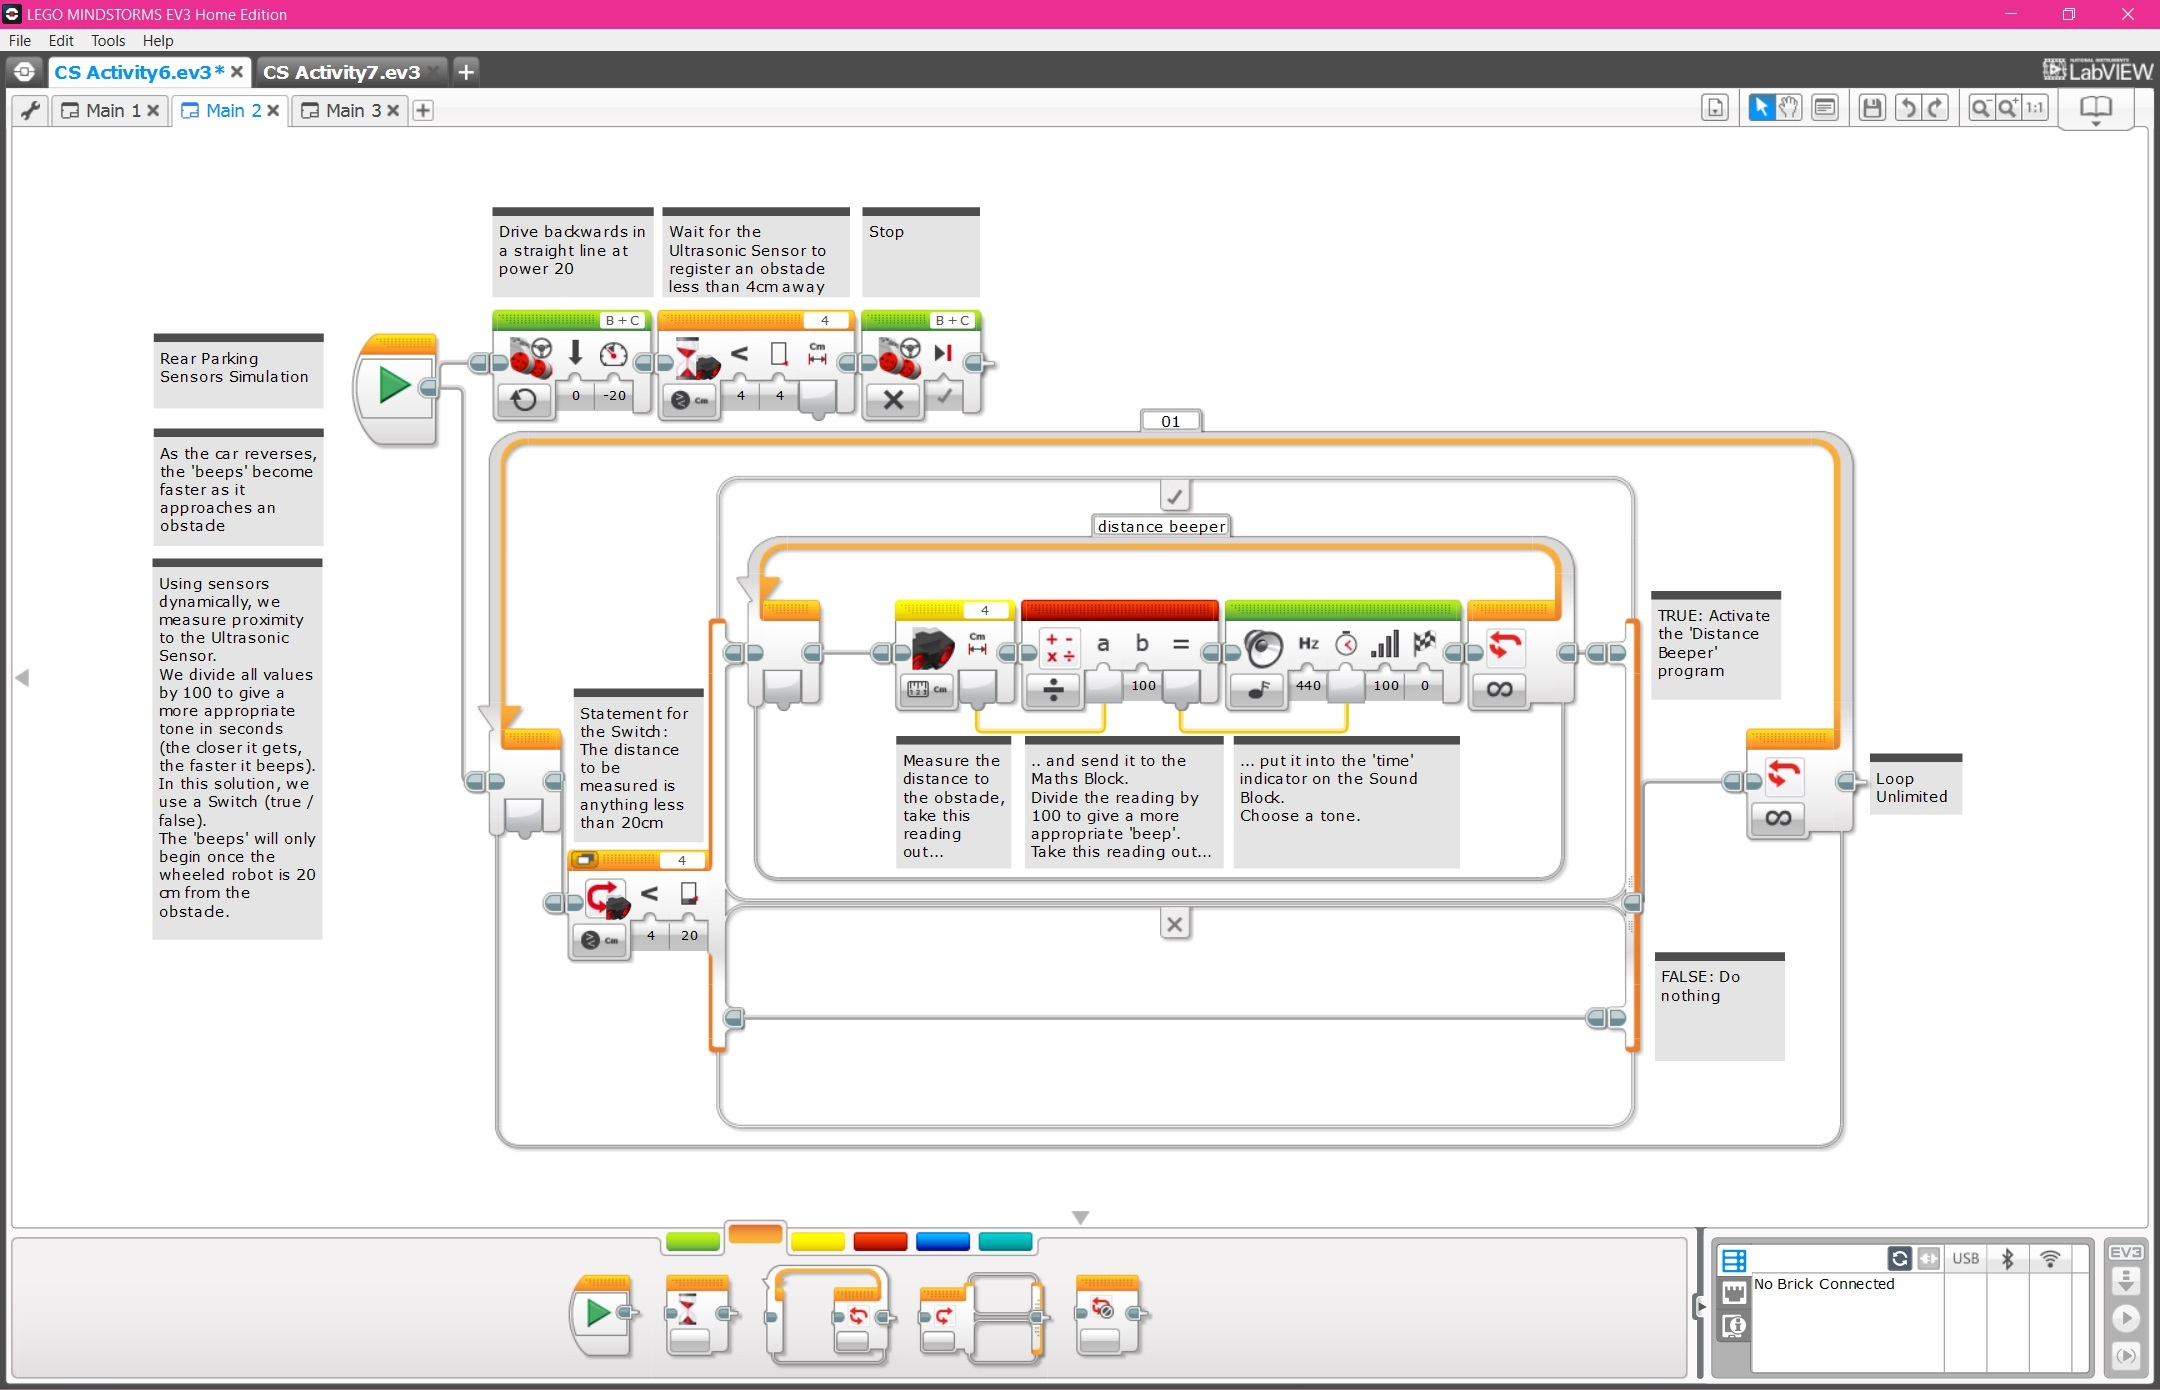
\includegraphics[width=0.5\textwidth]{Images/EV3ProgrammingSoftware.jpg}
  	\caption{A sample program in \enquote{EV3 Programming Software}}
  	\label{fig:ev3software}
  \end{center}
\end{figure}

\subsection{Puzzle-Solving with Algorithms}
\paragraph{•}
When it comes to playing games and solving puzzles, Google's AlphaGo Zero is the clear winner. Whilst Google's first Go-playing program defeated the world champion at Go, it took months of supervised learning from experts and reinforcement learning from self-play. The new version started \textit{tabula rasa} and was completely self-taught - it had no interaction with any humans, and uses no historical data. Through reinforced learning alone by simulating games against itself, it took three days to reach the level of AlphaGo and in forty days had surpassed any Go player's performance - human or artificial \cite{Silver2017}, \cite{Cellan-Jones2017}.
\paragraph{•}
When a computer solves a Cube (or any other similar puzzle), it does so by following set algorithms and rules until the solved state is achieved. Computers cannot use human-like instincts, so we often try to provide a heuristic to make the task simpler. These heuristics can be pre-computed data tables to reduce the amount of processing at run time, or a reduction in the original data set through elimination of certain data sets. In his 1997 paper on the use of pattern databases to increase solve efficiency, Richard Korf uses different heuristic functions and characterises how effective they are in reducing the number of moves in a solve sequence. His first method used an Iterative-Deepening A* algorithm, combined with the heuristic of the Manhattan distances from the edge cubies’ current position and orientation to that which is desired. This reduced the time required to solve a Cube at depth-14 to three days , however when increased to depth-18 the time increased exponentially to two hundred and fifty years. After a re-evaluation, Korf modified the heuristic by pre-computing the Manhattan distance of each cubie from all of its possible positions and orientations and storing the table in memory at run-time. This created a table of nearly ninety-million entries - which would have been bigger but was restricted by the available memory (the table was approximately forty-two megabytes). The newer heuristic reduced the time to search at depth-18 to less than four weeks - a reduction of ~99.97\%. Korf suggested that the speed of the algorithm used would increase linearly with the amount of memory available, meaning that if it were run today the depth-18 search would take under three hours \cite{Korf1997}.
\paragraph{•}
There have been many historical landmark algorithms since the Cube's inception in 1974. One of the earliest instances was created by Morwen Thistlethwaite circa 1981 and is based on group theory. Thistlethwaite's algorithm splits all possible positions of the cube into five groups of decreasing size as seen in Table 1. David Singmaster, Thistlethwaite's colleague at London South Bank University (then called Polytechnic of the South Bank), describes the methodology of the algorithm: \enquote{Once in $G_{i}$ , one only uses moves in $G_{i}$ to get into $G_{i+1}$. The ratio $|G_{i} |/|G_{i+1} |$  is called the index of $G_{i+1}$ in $G_{i}$.} Using this algorithm, Thistlethwaite proved that the maximum number of moves required to solve any valid position is fifty-two \cite{Singmaster1981}. This was the first development of God's Number, so named because it is the number of moves that an omniscient being would use to solve a Cube in the most efficient manner without failure. 

\begin{table}[h]
  \begin{center}
    \caption{Morwen Thistlethwaite's five groups for his algorithm \cite{Singmaster1981}}
    \label{tab:table1}
    \renewcommand{\arraystretch}{1.75}
    \begin{tabularx}{\textwidth}{ccX}
      \toprule
      \textbf{Group} & \textbf{Group Members} & \textbf{Summary}\\
      \midrule
      $G_0$ & $\langle L R, F, B, U, D\rangle$ & All valid positions \\
      $G_0$ & $\langle L, R, F, B, U2, D2\rangle$ & All positions that can be reached with quarter turns of the $L, R, F, B$ faces but only half turns of the $U, D$ slices \\
      $G_0$ & $\langle L, R, F2, B2, U2, D2\rangle$ & Positions reachable from quarter turns of $L, R$ and half turns of $F, B, U, D$\\
			$G_0$ & $\langle L2, R2, F2, B2, U2, D2\rangle$ & Positions only reachable from half turns of any face\\
      $G_0$ & $\{I\}$ & The goal state\\
      \bottomrule
    \end{tabularx}
  \end{center}
\end{table}
\renewcommand{\arraystretch}{1}

\begin{appendix}
\newpage  
\listoffigures
\listoftables
\newpage
\bibliographystyle{ieeetr}
\bibliography{library}
\end{appendix}
\end{document}